\documentclass[../template]{subfiles}

\newcommand{\idiff}{\ensuremath{I = \frac{dQ}{dt}}}

\begin{document}
\section{Dispositivi e Circuiti Elettronici}
La corrente elettrica $\idiff$ è generata da movimenti di carica. Il campo elettrico provoca lo spostamento di cariche dei materiali in esso.
\[
    \overline{J} = \sigma \overline{E}
\]
La densità di corrente elettrica $J$ dipende linearmente dal campo elettrico e dalla conducibilità elettrica del materiale.
Maggiore è il valore di $\sigma$, maggiore sarà la densità di corrente. I materiali isolanti hanno bassa conducibilità, ed i conduttori hanno alta conducibilità.

I semiconduttori sono materiali con conducibilità elettrica $\sigma$ variabile (ad esempio in funzione della temperatura).
Guardando il caso del componente resistenza, la corrente ai capi di essa dipende dall'inverso della costante $R$, quindi, a tensione costante, maggiore è la resistenza, minore è la corrente misurata ai due capi del componente.

\begin{figure}[h]
    \centering
    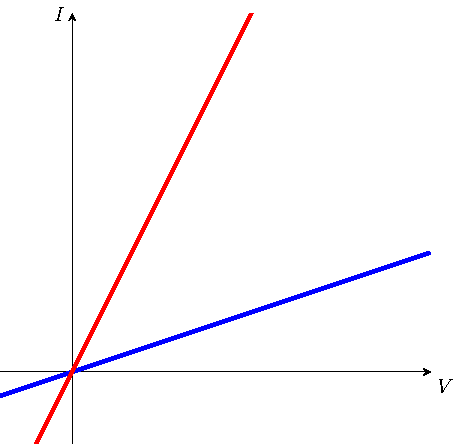
\includegraphics[width=.30\textwidth]{img/resistence-current}
    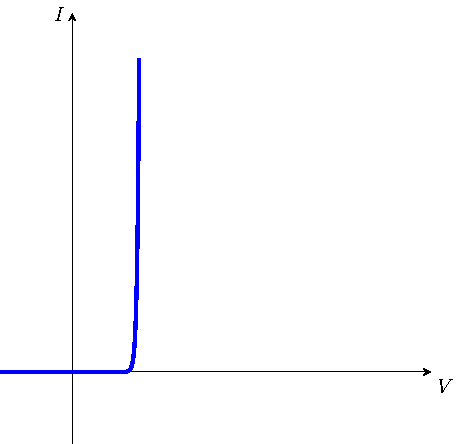
\includegraphics[width=.30\textwidth]{img/diode-current-graph}
\end{figure}
In figura sono riportate le relazioni corrente-tensione di una resistenza ed un diodo. È possibile osservare come il comportamento della corrente del diodo è completamente differente.

\subsubsection{Modello fisico}
Gli elettroni di ciascun materiale orbitano attorno ai rispettivi nuclei, in stato di equilibrio.
In stato equilibrio, gli elettroni di un materiale orbitano attorno al nucleo, la complessiva somma delle cariche risulta nulla.

Gli elettroni attratti dalla forza coulombiana, orbitano attorno al nucleo. Ad ogni orbita corrisponde una velocità di percorrenza,
quindi un'energia cinetica. L'ampiezza di ogni orbita dipende inversamente dal quadrato della distanza dal nucleo (formula forza di coulomb).
\\
In definitiva, possiamo

% TODO

Maggiore è la grandezza dell'orbita degli elettroni, maggiore è la veloci
Inoltre maggiore è la grandezza dell'orbita degli elettroni, maggiore è la velocità degli elettroni, quindi la loro energia cinetica.

All'ampiezza dell'orbita è quindi associato inversamente la forza attrattiva del nucleo, ed un'energia cinetica legata alla velocità di percorrenza.
\\
Possiamo quindi, gli elettroni interni ad un atomo generico in funzione dell'energia da essi posseduta, ottenendo un diagramma simile a quello in figura ..., distinta da diversi livelli

\begin{figure}[h]
    \centering
    \begin{tikzpicture}
        \draw[->] (0, 0) -- (0, 3)
            node[right]{$E$};

        \foreach \y in {.5, 1, ..., 2.5}
        {
            \draw (-3pt, \y) -- (+3pt, \y);
        }
    \end{tikzpicture}
\end{figure}

Ad ogni elettrone è dunque associato un livello sull'asse delle energie.
Per il principio di quantizzazione, dell'energia, non tutti i possibili livelli di energia sono possibili. L'asse quindi non è continua, ma quantizzata.

È importante notare che le orbite degli elettroni attorno agli atomi non sono descritte dalla meccanica classica, ma dalla meccanica quantistica, dove gli elettroni sono descritti attraverso forme sinusoidali.

Per questo motivo è possibile associare agli elettroni una lunghezza d'onda $\lambda$, dove nel caso di ipotesi stazionaria, è necessario che la circonferenza dell'orbita sia multiplo di $\lambda$.
\\
Questo spiega a grandi linee la presenza di valori permessi e proibiti sull'asse delle energie.

\subsubsection{Principio di esclusione di Pauli}
Ciascun livello energetico è occupabile al più da due elettroni (con spin opposto). In altre parole, il numero di elettroni che possono avere una certa distanza dal nucleo è finito.

Da questo è possibile dedurre che è possibile occupare interamente i livelli di energia.

Spostare corrente vuol dire spostare elettroni, cambiandone la velocità, quindi aumentandone l'energia cinetica, vincolata dai livelli di energia e dal principio di esclusione.

Per muovere un'elettrone quindi serve almeno l'energia per raggiungere il livello energetico libero più vicino.

Nel momento in cui due atomi diventino abbastanza vicini da interagire, quello che mi posso aspettare è che gli elettroni dei rispettivi atomi esercitino una forza repulsiva, con l'effetto di modificare l'orbita dei due elettroni.

Considerando quindi un unico diagramma energetico per il sistema dei due atomi, quello che ottengo è che i livelli non si sovrappongono ma si scostano leggermente, mantenendo comunque i principi di quantizzazione ed esclusione.

Generalizzando il discorso con un'interazione di $n$ atomi, otteniamo che ai precedenti livelli energetici, corrisponderà una moltitudine di livelli permessi, tra loro poco differenti, chiamata \textit{banda permessa}.
\\
I valori di energia tra due bande permesse, prendono il nome di \textit{banda proibita}.

È importante sottolineare che i valori interni alla banda permessa rispettano ancora il principio di esclusione e di quantizzazione, quindi è possibile che un'intera banda sia occupata da elettroni.

In condizione di quiete, gli elettroni tendono spontaneamente ad occupare i livelli più bassi, ad energia minore.

La statistica di fermi indica un valore limite (\textit{Livello di Fermi}) che indica, in assenza di perturbazione, in termini probabilistici, tutti i livelli che sotto tale valore risultano occupati.

La posizione in cui ricade il livello di Fermi, indica il tipo di materiale:
\begin{itemize}
    \item Se è interno ad una banda permessa, è richiesta poca energia per spostare gli elettroni ad il livello energetico successivo, quindi il materiale è conduttore.
    \item Se è in banda proibita, il materiale è isolante.
    \item Se è in una banda proibita, ma l'energia necessaria a raggiungere la banda permessa successiva è ragionevole, il materiale è semiconduttore.
\end{itemize}

Quindi i materiali isolanti hanno un livello di tolleranza all'energia che ricevono, prima di manifestare un fenomeno di scarica.

\subsubsection{I semiconduttori}
Nei materiali semiconduttori, la prima banda permessa sopra il livello di fermi prende il valore di banda di conduzione,
mentre la prima al di sotto prende il nome di banda di valenza.

Quando elettroni passano dalla banda di valenza alla banda di conduzione, lasciano spazi in banda di valenza.
Con l'aumento dell'energia fornitagli, aumentano il numero di elettroni che passano in banda di conduzione.

Possiamo considerare la banda di valenza come una seconda banda di conduzione.

% seconda lezione
La distanza dal nucleo cresce col crescere dell'energia, gli elettroni sullo strato di valenza sono quelli più distanti dal nucleo.
La forma del reticolo di atomi è determinata dal numero di elettroni disponibili a collegarsi agli atomi vicini.
Tutti i materiali semiconduttori sono materiali della quarta colonna della tavola periodica, e possiedono quattro elettroni in orbita di legame.

Il semiconduttore utilizzato maggiormente è il silicio.

In alternativa agli elementi della tavola periodica è possibile formare delle leghe tra elementi della terza e quarta colonna o quarta e quinta, come arseniuro di gallio.

Schematizzando il reticolo del silicio su una mappa in bidimensionale (figura ?)
La promozione di un'elettrone da banda di valenza a banda di conduzione, indebolisce il legame con il nucleo originario, rendendo possibile spostare gli elettroni internamente al reticolo applicando un campo magnetico esterno.
Tali elettroni vengono definiti come elettroni liberi.

Il materiale in condizione di quiete è neutro, ovvero ha tanta carica positiva quanta negativa. Al momento in cui un'elettrone libero esce da una regione, quella regione non ha più carica nulla ma leggermente positiva. Possiamo quindi immaginare il moto dell'elettrone come uno spostamento di carica nello spazio, quindi una corrente.
\\
Lo spazio lasciato vuoto dall'elettrone, è successivamente occupato da altri elettroni liberi. Creando uno spostamento a catena degli elettroni.

Alla banda di conduzione è associato il movimento di una carica negativa, alla banda di valenza è associato il movimento della lacuna, carica positiva generata dallo spostamento dell'elettrone.

In un conduttore esiste solo un tipo di portatore di carica (elettroni), mentre nei semiconduttori esistono portatori di carica positiva e portatori di carica negativa.

È possibile modellare il movimento della lacuna come il movimento di una fittizia particella fisica, dotata di massa (maggiore di quella dell'elettrone perché si muove più lentamente)

Per misurare la corrente è necessario conoscere la quantità di elettroni e lacune in un determinato volume.
Indicheremo quindi con $n$ il numero di elettroni per unità di volume \footnote{Misurata per numero di elettroni per centimetro cubo}.
Analogamente definiamo la concentrazione di lacune con $p$ come il numero di lacune per unità di volume.

Per densità di carica degli elettroni si calcola con $-qn$, mentre per lacune $qn$.
Ad ogni elettrone libero in banda di valenza, corrisponde una lacuna in banda di conduzione, quindi necessariamente all'equilibrio $p = n$.

Possiamo definire come evento di generazione il momento in cui un'elettrone abbandona la banda di valenza generando una lacuna, mentre il fenomeno duale, il passaggio da banda di conduzione a bassa di valenza viene chiamato evento di ricombinazione.

Indichiamo con $G$ il numero di coppie elettrone-lacune generate nell'unità di volume e nell'unità di tempo. Il tasso di ricombinazione è indicato con $R$.

All' equilibrio $n = p = n_i(T)$ e $R = G\ge 0$ il numero di elettroni e lacune in banda di valenza costante prende il nome di $n_i$ (concentrazione intrinseca del materiale).

Sostituendo ad alcuni atomi di silicio, con atomi della 5a colonna, as es fosforo. In questo modo avendo un'elettrone di legame in più (ed un protone in più), siccome i legami sono tutti occupati con gli atomi di silicio adiacenti, otteniamo un'elettrone che non contribuisce ad alcun legame nel reticolo.
\\
La sostituzione di alcuni atomi di silicio con atomi della 3a o 5a colonna prende il nome di drogaggio.

La rara sostituzione di atomi di silicio, non varia la struttura del reticolo cristallino originario.

L'elettrone nella fascia più esterna non essendo legato agli altri se riceve energia sufficiente può liberarsi e comportarsi come una carica negativa mobile. È ancora vero che lascia alle sue spalle una carenza di carica negativa, ma la carica positiva è associata alla presenza del protone nel nucleo e non è in grado di spostarsi.
In questo caso si genera un'elettrone mobile, senza generare lacune mobili. In questo caso $p \neq n$. Gli atomi della quinta colonna prendono quindi il nome di atomi droganti di tipo donatore.

Tutto questo è rappresentabile nel diagramma delle energie inserendo un livello "donatore" interno alla banda proibita permettendo che l'evento di liberazione dell'elettrone richieda meno energia, rendendolo ancora più probabile a temperatura ambiente.
\\
Chiameremo $N_D$ la concentrazione di atomi donatori.
%, e per mantenere la struttura del cristallino $N_D \ll 10^{22}$.

Analogamente prendendo un' elemento della terza colonna (es. boro) nel reticolo viene rimosso un legame, fornendo energia al reticolo e spostando elettroni, essi andranno ad occupare del legame mancante, generando lo spostamento di una carica positiva.
La carica negativa è fissa perché legata alla struttura del boro.

Chiameremo il boro atomo accettore, perché capace di ionizzare il reticolo negativamente. Con $N_A$ indicheremo la concentrazione degli atomi accettori per unità di volume. Interpretando l'evento sul diagramma energetico, sarebbe come un livello energetico che ricade nella banda proibita molto vicino alla banda di valenza. Generando una lacuna mobile in tale banda.

In questo caso $n < p$.

\subsubsection{Terza Lezione}
Abbiamo interpretato il diverso comportamento delle due bande, elettroni liberi che si muovono tra livelli energetici nella banda di conduzione, e lacune alle quali è associato un significato di carica positiva mobile.
\\
In un materiale intrinseco, elettroni e lacune sono creati sempre in coppia, quindi necessariamente la concentrazione di elettroni e lacune sono uguali alla concentrazione intrinseca, dipendente dalla temperatura.

Inoltre in condizioni di equilibrio il tasso di generazione $G$ e di ricombinazione $R$ devono essere uguali.

La relazione tra elettroni e lacune in banda di valenza può essere modificata attraverso drogaggi con atomi donatori o accettori. La concentrazione di elettroni-lacune di materiali drogati prende il nome di \textit{concentrazione intrinseca}

Supponendo di conoscere la concentrazione tra atomi donatori ed accettori, calcoliamo ora i nuovi valori di $p$ ed $n$ interni al materiale.

Osservando il caso della concentrazione intrinseca, osserviamo che necessariamente vale il prodotto $pn = n_i^2$. Questa relazione è valida non solo per materiali intrinseci, ma anche per materiali estrinseci.

Possiamo pensare che il tasso di generazione $G$ sia dipendente unicamente dalla temperatura: $g(T)$.
Mentre il tasso di ricombinazione $R$, è logico pensare che dipenda dal numero portatori di carica e dalla temperatura: $R = pnr(T)$.
\\
$G$ non dipende dal numero di portatori di carica, in quanto per evitare che si verifichi il fenomeno,
tutti gli elettroni in banda di valenza, dovrebbero essere spostati in banda di conduzione. Il che è molto improbabile se
lavoriamo a temperatura ambiente.

Ricordandoci che in condizioni di equilibrio $G = R$, otteniamo che $g(T) = pnr(T)$. Quindi $pn = g(T)/r(T) = f(T)$ è dipendente unicamente dalla temperatura. Quindi a temperatura costante il valore $pn$ è costante e vale $n_i^2$.

Inoltre se è vero che a livello globale la quantità di carica positiva equivale alla carica negativa, allora la densità di carica $\rho$ in tutto il volume è costante e pari a $0$.

\[
    \rho = -q n + qp  + qN_D -q N_A = q (p -n + N_D - N_A) = 0
\]
La densità di carica dipende dal numero di elettroni $n$ e lacune $p$ con rispettiva carica, ed il numero di atomi accettori e donatori interni ad un materiale, ad ognuno dei quali è associata rispettivamente una carica fissa in modulo $q$.
\\
Unendo la relazione con $pn = n_i$, ricaviamo:
\[
    n = \frac{(N_D - N_A) \pm \sqrt{(N_D - N_A)^2 + 4 n_i^2}}{2}
\]
Siccome è evidente che non può valere il segno meno in quanto condurrebbe ad un valore di $n$ negativo, ottengo un'espressione del valore di $n$ dipendente solo da valori noti.
\\
Con questo ragionamento otteniamo anche il valore di $p$:
\[
    p = \frac{(N_A - N_D) + \sqrt{(N_A - N_D)^2 + 4 n_i^2}}{2}
\]

Dalle espressioni si può osservare come compare sempre la differenza dei valori $N_D$ ed $N_A$, il fenomeno prende il nome di principio di compensazione, il quale dice che non è importante il singolo valore di $N_D$ ed $N_A$, quello che conta è sempre la loro differenza.


Nel caso di una concentrazione con forte sbilanciamento, es $N_D \gg N_A \gg n_i$, nelle equazioni in precedenza, posso trascurare i termini $N_A$ ed $n_i$, ottenendo $n = N_D$.
Quindi se la concentrazione del drogante è molto maggiore rispetto alla concentrazione intrinseca, allora la concentrazione di elettroni è dovuta praticamente solo ad esso.
Siccome vale $pn = n_i^2$, abbiamo che $p = n_i^2 / N_D$. Segue che il trasporto della carica, avviene quasi unicamente attraverso elettroni.
\\
Chiameremo questo materiale "estrinseco di tipo n", ad indicare la larga prevalenza degli elettroni.

Posso effettuare gli stessi ragionamenti nel caso duale ($N_A \gg N_D \gg n_i$), ottenendo $p = N_A$ e $n = n_i^2 / N_A$.
Chiameremo questo materiale "estrinseco di tipo p".

\subsubsection{Studio conduzione materiale uniforme, estrinseco di tipo n}

Conoscendo la conduzione del materiale $n \approx N_D$, ed indicando con $S$ la sezione trasversale del materiale, indicheremo $J = I/S$.
Ricordando che $I = dQ/dt$, otteniamo:
\[
    J = \frac{1}{S}\frac{dQ}{dt}
\]
Per via delle forze repulsive interne al materiale, si può vewdere sperimentalmente che gli elettroni si muovono a velocità costante $V_n = -\mu_n E$, in direzione opposta al campo elettrico, con $\mu_n$ costante di mobilità elettronica.

Il percorso che percorre una singola particella in un piccolo intervallo di tempo è esprimibile quindi come $dx = -\mu_n E dt$.
\\
La carica $dQ$ è quella che nello stesso intervallo di tempo $dt$ attraversa la sezione del materiale, è possibile pensarla come $nq S dx$ (carica del numero di portatori nel volume $Sdx$).

Quindi la densità $J$ è esprimibile come:
\[
    \begin{cases}
        \frac{dx}{dt} = \mu_n E
        \\
        J = \frac{1}{S} \frac{dQ}{dt}
        \\
        Q = qnS dx
    \end{cases}
    \Rightarrow
    J_n = \frac{1}{\cancel{S}} \frac{qn\cancel{S} \mu_n E \cancel{dt}}{\cancel{dt}} = qn\mu_n E
\]
Vale ancora la relazione di ohm in forma locale $J = \sigma E$, con $\sigma = qn \mu_n = q \mu_n N_D$.
È possibile concludere che $N_D \propto \sigma$. Quindi possiamo variando dinamicamente il valore di $N_D$ si può ottenere un conduttore o un isolante.

Quindi solo variando il valore di $N_D$ in una parte del materiale posso formare due regioni conduttive, separate da una isolante.

\subsubsection{Conduzione materiali estrinseci di tipo p}
Con ragionamento del tutto analogo al precedente, si ottiene che la velocità di mobilità delle lacune è pari a $V_p = \mu_p E$.
Nel dettaglio $\mu_p \approx \frac{2}{3} \mu_n$, sottolineando che le lacune si comportano come particelle fittizzie che si muovono più lentamente degli elettroni.

Ottenendo
\[
    J_p = \frac{1}{S}\frac{qp\mu_pESdx}{dt} = qp\mu_p E
\]
In questo caso la conducibilità elettrica è determinata da $N_A$.

La totale conducibilità elettrica è possibile esprimerla come $J = J_n + J_p$. $J$ conta la quantità di carica che attraversa la sezione, quindi gli elettroni portano contributo positivo muovendo carica negativa in senso opposto, e le lacune portano contributo positivo.
\[
    J = J_n + J_p = qn\mu_n E + qp \mu_p E
\]
\subsubsection{Materiale drogato non uniformemente}

Nel caso in cui il campo elettrico esterno sia nullo, gli elettroni si spostano ugualmente per il moto browniano.
Possiamo pensare alla carica $dQ$ come $dQ_1 - dQ_2$ ovvero la carica dovuta agli elettroni che escono dalla sezione di volume, e la carica degli elettroni entranti nella sezione di volume.
Chiamata quindi $n_1$ la quantità di elettroni esterni al volume, e $n_2$ la quantità di elettroni interni; siccome le cariche hanno un 50\% di probabilità di entrare nel volume, si possono esprimere le cariche come:
\begin{align*}
    dQ_1 = -\frac{q n_1 dV}{2}\\
    dQ_2 = -\frac{q n_2 dV}{2}
\end{align*}
Ricordando che il volume $dV = S V_{th} dt$ ($V_{th}$ velocità termica) si ottiene che:
\[
    J_n = \frac{1}{S} \frac{-qn_1 S V_{th} dt + qn_2 S V_{th} dt}{2dt}  = q(n_2 - n_1) V_{th} \neq 0
\]
Ma siamo giunti ad un assurdo, in quanto avremmo trovato un modo per generare corrente senza spendere energia.

Effettuando i calcoli più accuratamente è possibile ottenere $J_n = q D_n \frac{dn}{dx}$. Quello che accade è il fenomeno della diffusione, infatti tende a muovere la carica, dalla regione di concentrazione più alta a quella più bassa. Il sistema evolve verso una distribuzione uniforme.
\\
Lo spostamento degli elettroni lascia cariche positive nella regione con maggior carica negativa, portando una carica negativa nell'altra regione.

Otteniamo quindi un campo elettrico nella direzione della regione con meno cariche negative, pari a $F = -qE$.

\subsection{Lezione 4}
% 17.03
Analogamente al caso precedente, studiamo un materiale estrinseco di tipo p, la cui concentrazione di lacune non è costante, ottenendo:
\[
    J_p = \frac{1}{S}\frac{d(Q_1 - Q_2)}{dt} = \frac{q(p_1 - p_2) V_{th}}{2}
\]
contrariamente al caso degli elettroni, se $p_2 > p_1$ otteniamo $J_p < 0$.
In questo, effettuando i calcoli in maniera più accurata, otterremo che $J_p = -qD_p \frac{dp}{dx}$.

Abbiamo introdotto quindi i funzionamenti di tipo ohmico: $J_n = q\mu_n n E$ e $J_p = q \mu_p p E$, la cui direzione è concorde;
ed un meccanismo di tipo diffusivo: $J_n = q D_n \frac{dn}{dx}$ e $J_p = -qD_p \frac{dp}{dx}$, la discordanza di segno è dovuta al bilanciamento della carica.

Non possiamo considerare i due funzionamenti come uno indipendente dall'altro, in quanto porterebbe a conclusioni assurde, esprimiamo quindi la combinazione degli effetti:
\begin{align*}
    J_n = q \mu_n n E + q D_n \frac{dn}{dx} \\
    J_p = q \mu_p p E + q D_p \frac{dp}{dx}
\end{align*}

Quindi un conduttore prevede un solo meccanismo di trasporto di carica, per un meccanismo unicamente di tipo ohmico. In un semiconduttore teniamo conto di due specie di carica e di due specie di carica e due diversi meccanismi di trasporto di carica: trasporto ohmico e diffusivo.

Il modello prende infatti il nome di ohmico-diffusivo (\textit{drift-diffusion}).

$D_n$ indica la reattività dell'elettrone alla temperatura.
\[
    D_n = \frac{kT}{q} \mu_n
\]
Analogamente $D_p = \frac{kT}{q}\mu_p$. Queste prendono il nome di relazioni di Einstein, dove $k$ è la costante di Boltzmann, $q$ è la carica dell'elettrone e $T$ è la temperatura.

Quello che dicono queste relazioni è che il coefficiente di diffusione e la mobilità dell'elettrone, sono legate.
Ricordando che la mobilità degli elettroni è superiore a quella delle lacune, analogamente il fattore $D_n$ è maggiore di $D_p$
% 37:50

Ricordandoci che $E = -\frac{d\phi}{dx}$
prendiamo in considerazione, un materiale, tale per cui la concentrazione varia in base alla coordinata $x$: $n(x)$.
Siccome il campo elettrico $E$, costante ed indipendente dalla posizione $x$, prendiamo un punto $x_1$ interno al materiale e lo usiamo come origine per misurare il campo elettrico. In tale punto avremo che $\varphi = 0$, $n_0$ e $p_0$.

Allo stesso identico modo posso scegliere un punto $x_2$, caratterizzato da un $\varphi(x)$, $n(x)$ e $p(x)$.

All'equilibrio $pn = n_i^2$, otteniamo che, dalla funzione di $J_n = q \mu_n  n E + q D_n \frac{dn}{dx} \approx 0$, otteniamo:
\[
    \frac{kT}{nq} \frac{dn}{dx} = \frac{d\varphi}{dx}
\]

Integrando la relazione sui margini $\varphi(0)$ e $\varphi(x)$, ottengo:
\[
    \varphi(x) = \frac{kT}{q} \ln \frac{n(x)}{n_0}
\]
Da cui
\[
    n(x) = n_0 e^{\dfrac{q\varphi(x)}{kT}}
\]
Inoltre dalla relazione $p(x) n(x) = n_i^2$, otteniamo la relazione duale $p(x) = p_0 e^{-q\varphi(x) / kT}$ la inversa $\varphi(x) = - \frac{kT}{q} \ln \frac{p(x)}{p_0}$.

% maxwell
Dalle equazioni di Maxwell, per i materiali uniformi: $\frac{d^2 \varphi}{dx} = -\frac{\rho}{\varepsilon}$
\subsection{Ragionamento su struttura diversamente drogata}
Supponiamo un unico cristallo di semiconduttore, drogato per metà in con atomi accettori, e per metà con atomi donatori.
Il materiale prende il nome di giunzione pn.


\subsubsection{Studio della struttura all'equilibrio}

Supponiamo una differente distribuzione di atomi accettori e donatori. Prendendo quindi come origine il punto intermedio tra le due giunzioni, otteniamo:

\begin{figure}[h]
    \centering
    \begin{tikzpicture}
        \begin{axis}[xlabel=$x$, ylabel=$$, ymin=-1, ymax=4]
            \addplot[domain=-5:0, red]{0};
            \addplot[domain=0:5, red]{2};
            \addplot[domain=-5:0, blue]{2.5};
            \addplot[domain=0:5, blue]{0};

            \draw (2, 2) node[red, above]{$N_D$}
                (-2, 2.5) node[blue, above]{$N_A$};
        \end{axis}
    \end{tikzpicture}
\end{figure}

Supponiamo che il dispositivo sia abbastanza lungo, da supportare l'ipotesi che dopo una certa distanza, l'effetto della giunzione risulti trascurabile, in modo che sia possibile esprimere le relazioni dei due estremi indipendentemente.
Quindi, che esistano due coordinate $w_p$ e $w_n$, che oltre a quelle coordinate, le due regioni si comportano come regioni uniformemente drogate di tipo $p$ ed $n$.


\begin{tcolorbox}[title={Zona neutra p}]
    Per $x < -w_p$, la popolazione di portatori maggioritaria sono le lacune, quindi $p = N_A$ e $n = \frac{n_i^2}{N_A}$
    \begin{align*}
        \rho = q (\cancel{N_D} - N_A + p - \cancel{n}) \approx  0\\
        J_p = q \mu_p p E - q D_n \frac{dp}{dx} = 0
    \end{align*}
    Essendo la densità di carica pari a 0, e la variazione di atomi portatori nulla, allora necessariamente $E = 0$

    Siccome $E$ dipende dalla derivata di $\varphi$ rispetto ad $x$ allora $\varphi$ è costante. Prendiamo questo valore, come valore di riferimento, per i successivi $\varphi$, quindi $\varphi = 0$.
\end{tcolorbox}
\begin{tcolorbox}[title={Zona neutra n}]
    Per $x > w_n$, $n = N_D$ e $p = \frac{n_i^2}{N_D}$. Inoltre $\rho = q (N_D - n) \approx 0$.
    \[
        J_n = q \mu_n n E + q D_n \frac{dn}{dx} = 0
    \]
    Per analogo ragionamento $E = 0$ e $\varphi$ è costante, calcolabile attraverso la formula
    \[
        \frac{kT}{q} \ln \frac{n(x)}{n_0} = \frac{kT}{q} \ln \frac{N_D N_A}{n_i^2}
    \]
    Indicheremo questo valore con $\Psi_B$. Siccome i valori di $N_D$ ed $N_A$ sono entrambi molto maggiori di $n_i$, allora $\Psi_B$ è positiva e molto maggiore di 1.
    Inoltre siccome dipende dal logaritmo di $N_D$ ed $N_A$, per variazioni di quest'ultimi è assimilabile ad una costante.
\end{tcolorbox}
\begin{tcolorbox}[title={Regione svuotata}]
    Per $-w_p < x < w_n$, ipotizzando che il potenziale sia monotono in questo intervallo, possiamo presupporre che $0 < \varphi(x) < \Psi_B$.

    Quindi in tutto l'intervallo $\varphi(x) > 0$, da cui moltiplicando per la quantità positiva $\frac{q}{kT}$, otteniamo
    \[
        p_0 e^{-\frac{q\varphi}{kT}} \ll p_0 = N_A
    \]
    Il cui primo termine è $p(x)$.
    Analogamente, da ipotesi di funzione monotona, posso dire che $\varphi(x) < \Psi_B$, e moltiplicandola per la stessa quantità positiva $\frac{q}{kT}$ ottengo:

    \[
    n(x) = n_0 e^{\frac{q\varphi(x)}{kT}} \ll n_0 e^{\frac{q\Psi_B}{kT}} = N_D
    \]

    Da cui i valori di $n$ e $p$ sono rappresentati graficamente da valori prossimi a 0.
\end{tcolorbox}
\begin{tcolorbox}[title={Regione svuotata e regione di carica}]
    Per $-w_p < x < 0$
    La densità di carica non sarà più nulla, ma siccome $p(x) \ll N_A$, $n(x) \ll N_D$, in base all'intervallo in cui mi trovo, per la relazione $\rho = q(N_D - N_A + \cancel{p} - \cancel{n})$, la densità di carica potrà valere $-qN_A$ o $qN_D$.
    Per la relazione di poisson: $\frac{dE}{dx} = -\frac{\rho}{\varepsilon}$. Sostituendo rispettivo valore di $\rho$ ed integrando nei relativi estremi, si ottiene il campo elettrico:
    \[
        E = - \frac{qN_A}{\varepsilon} (x + w_p)
    \]
    Nel caso particolare $E(0^-) = \dfrac{-qN_A w_p}{\varepsilon}$

    Dalla relazione $E = -\frac{d\phi}{dx}$, integrando sugli estremi si ottiene:
    \[
        \varphi(x) = \frac{qN_A}{\varepsilon}\frac{{(x + w_p)}^2}{2}
    \]
    con $\varphi(0^-) = \frac{qN_A}{2\varepsilon}w^2_p$
\end{tcolorbox}
\begin{tcolorbox}[title={}]
    Per $0 < x < w_n$, con analoghi ragionamenti, $\rho = qN_D$
    ed il campo elettrico $E$ e potenziale $\phi$ saranno rispettivamente:
    \begin{align*}
        &E(x) = \frac{qN_D}{\varepsilon} (x - w_n) & E(0^+) = - \frac{qN_D}{\varepsilon} w_n\\
        &\phi(x) = \Psi_B - \frac{qN_D}{2\varepsilon} {(x - w_n)}^2 & \psi(0^+) = \Psi_B - \frac{qN_D}{2\varepsilon} w_n^2
    \end{align*}
\end{tcolorbox}

\begin{figure}[h]
    \centering

    \def\wp{-1.2}
    %\def\wn{2}
    \def\eps{1}
    \def\fb{2}
    \def\wn{sqrt(2*\fb/\eps - \wp*\wp)}

    \begin{tikzpicture}
        \begin{axis}[width=.33\textwidth, xlabel=$x$, ylabel=$$]
            \addplot[domain=\wp:5, red]{0};
            \addplot[domain=-5:\wp, red]{1.6};
            \addplot[domain=-5:\wn, blue]{0};
            \addplot[domain=\wn:5, blue]{1.5};
            \draw
                (\wp-1, 1.6) node[above, red]{$p$}
                (3, 1.6) node[above, blue]{$n$}
                ;
        \end{axis}
    \end{tikzpicture}
    \begin{tikzpicture}
        \begin{axis}[width=.33\textwidth, xlabel=$x$, ylabel=$\rho$]
            \addplot[domain=-5:\wp, blue]{0};
            \addplot[domain=\wp:0, blue]{-1};
            \addplot[domain=0:\wn, blue]{1};
            \addplot[domain=\wn:5, blue]{0};
        \end{axis}
    \end{tikzpicture}
    \begin{tikzpicture}
        \begin{axis}[width=.33\textwidth, xlabel=$x$, ylabel=$E$]
            \addplot[domain=-5:\wp, blue]{0};
            \addplot[domain=\wp:0, blue]{\eps*(- x + \wp)};

            \addplot[domain=0:\wn, blue]{\eps*(x - \wn)};
            \addplot[domain=\wn:5, blue]{0};
        \end{axis}
    \end{tikzpicture}
    \begin{tikzpicture}
        \begin{axis}[width=.33\textwidth, xlabel=$x$, ylabel=$\phi$]
            \addplot[domain=-5:\wp, blue]{0};
            \addplot[domain=\wn:5, blue]{\fb};
            \addplot[domain=\wp:0, blue]{\eps * ((x - \wp)^2)/2};
            \addplot[domain=0:\wn, blue]{\fb - \eps * ((x - \wn) ^2 /2)};
        \end{axis}
    \end{tikzpicture}
\end{figure}

Se è presente una corrente diffusiva, è presente anche una corrente opposta di trascinamento ohmico. La regione $-w_p < x < 0$ è sede di carica negativa fissa, e la controparte $ 0 < x < w_n$ è ricca di atomi droganti, che avendo donato elettroni per effetto di diffusione, portano una regione di carica positiva fissa.

Le cariche fisse positive e negative, rappresentano un dipolo di carica, e generano un campo elettrico rivolto verso la regione p.
Per sostenere tale campo elettrico è necessaria una differenza di potenziale.

La condizione di equilibrio è raggiungibile in due modi: o sia la componente ohmica e diffusiva sono nulle, o opposte.
In particolare lo spostamento di elettroni per diffusione forma un campo elettrico ohmico che all'equilibrio è uguale ed opposto.

$\Phi_B$ prende infatti il nome di potenziale di barriera, perché è necessario a sostenere il campo elettrico necessario a bilanciare la diffusione.

\subsubsection{Lezione 5 - 12}
Il modello appena analizzato si basa sull'esistenza di due coordinate $w_p$ e $w_n$, che discriminano regioni tra vicine e lontane alla giunzione di carica.

Osservando che $E(0-) = E(0+)$, dalle relazioni, si ricava che $-qN_A w_p = -qN_D w_n$, considerato che dal grafico della densità di carica $\rho$, $qN_A$ e $w_p$ sono base ed altezza del rettangolo

L' equazione esprime l'uguaglianza tra le due aree dei rettangoli del primo e terzo quadrante.
Integrando quindi densità di carica sul volume, moltiplico entrambi i rettangoli per la sezione trasversale $S$, ottengo che il volume dei due cilindri $w_p S$, moltiplicato alla densità di carica $qN_A$, ottenendo le cariche $Q_p$ e $Q_n$ associate alla regione svuotata.

In questa regione quindi, il dispositivo si comporta come un condensatore. La differenza è che la carica del condensatore è concentrata su due armature, questa carica è distribuita nel volume.

Questa relazione esprime che $w_p$ e $w_n$ sono legati tra loro da una relazione.


Ponendo l'uguaglianza tra le due formule del potenziale $\Psi$ nell'origine, otteniamo:
\[
    \Psi_B = \frac{q}{w \varepsilon} \big(N_A \cdot \frac{N_D^2}{N_A^2} + N_D \big) w_n^2 = \frac{qN_D^2}{2\varepsilon} \big( \frac{1}{N_A} + \frac{1}{N_D} \big) w_n^2
\]

Da cui si ricava il valore di $w_n$ come:
\[
w_n = \frac{1}{N_D} \sqrt{\frac{2\varepsilon \Psi_B}{q\big(\frac{1}{N_D} + \frac{1}{N_A}\big)}}
\]
e $w_p$ segue dalla relazione $w_p N_A = w_n N_D$.

Dipendentemente dalla concentrazione dei droganti, i valori di $w_p$ e $w_n$ assumono valori dell'ordine di $10^{-6} m$ o inferiori, quindi l'ipotesi di esistenza delle zone neutre, sufficientemente lontane dalla giunzione, è soddisfatta appena le dimensioni fisiche del dispositivi eccedono i decimi di micron.

% 21min
L'alta densità di lacune nella regione $p$, tende per effetto di diffusione, a muoversi verso la regione $n$.
Allo stesso tempo, l'alta densità di elettroni tendono a spostarsi nella regione $p$. Per questa condizione la corrente non può essere nulla. Difatti ad un dipolo di carica è associato un campo elettrico, col verso rivolto dalla carica positiva, alla negativa.

Il campo elettrico è intrinseco. Le lacune si muovono per effetto di diffusione da $p$ ad $n$, gli elettroni si muovono per il campo elettrico da $n$ a $p$ per effetto di trascinamento.

L'effetto del campo elettrico contrasta il fenomeno della diffusione, ed all'equilibrio le due componenti sono bilanciate.
Nell'ipotesi in cui non ci sia trascinamento, ci sarebbe solo diffusione, non contrastata, portando una corrente non nulla, contraddicendo l'ipotesi di equilibrio.

Analogamente se la regione svuotata si estendesse infinitamente, non si avrebbe diffusione in quanto non variabile, ma solo il trascinamento ohmico. I due fenomeni quindi esistono insieme.

La diffusione agisce sulle lacune, portandole dalla regione $p$, alla $n$, per questo prende il nome di diffusione di portatori maggioritari. Il trascinamento, invece agisce sugli elettroni: i portatori minoritari.

\[
    \Psi_B \approx 0.5 V
\]
Questa differenza di potenziale non è in grado di fornire energia internamente ad una maglia, è la reazione intrinseca del materiale che si oppone generare corrente senza sorgente di energia.

Ipotizzando quindi di cortocircuitare la giunzione, per lo stesso motivo per cui esiste una differenza di potenziale tra le due regioni polarizzate differentemente, esistono due differenze di potenziale "di contatto" ai capi della giunzione, collegata al filo conduttore in metallo.

\subsubsection{Calcoli in regione dinamica}
Spostandoci dalla condizione di equilibrio, ovvero applicando un generatore di tensione alla maglia, ne consegue che la corrente interna non è nulla.
%42

I due potenziali di barriera $\Psi_{cn}$ e $\Psi_{cb}$, possono essere considerati costanti, e uguali alla differenza di potenziale, calcolata precedentemente in condizione di equilibrio.
Questa condizione prende il nome di "condizione di contatto ohmico", ovvero che la tensione è indipendente dalla corrente.

Quando un flusso di carica attraversa una regione $p$ o $n$, la conducibilità elettrica $\sigma = q N_A \mu p$. Dalla conducibilità si ricava la resistività $\rho$ come $\rho = \frac{1}{\sigma}$, e quindi la resistenza vale: $R = \rho \frac{l}{S}$, considerando in questo modo la regione $p$ come una resistenza. Analogo ragionamento vale per la regione $n$.

Alle regioni $p$ ed $n$ corrisponde quindi una differenza di potenziale: $\Psi_p$ e $\Psi_n$.

L'equazione di kirkoff alla maglia diventa quindi:
\[
    V + \Psi_{cp} - \Psi_p - \Psi_B - \Psi_n - \Psi_{cn} = 0
\]

Con $V$ pari alla tensione applicata alla maglia. Prendendo come ipotesi che le differenze di potenziale $\Psi_p$ e $\Psi_n$ siano molto più piccole del potenziale di barriera $\Psi_b$, possiamo semplificare l'equazione a $V + \Psi_{cp} + \Psi_B - \Psi_{cn} = 0$.

Questa ipotesi di semplificazione è quindi anche una condizione di validità dell'equazione ottenuta.

Ricordando che i due potenziali siano costanti, all'equilibrio: $0 + \Psi_{cp0} + \Psi_{B0} - \Psi_{cn0} = 0 $, da cui $\Psi_{B0} = \Psi_{cn0} - \Psi_{cp0} = \Psi_{cn} - \Psi{cp}$.

Riportato il risultato ottenuto all'equazione precedente:
\[
    V - \Psi_{B0} + \Psi_B = 0
\]

Sotto ipotesi di validità, la barriera di potenziale $\Psi_B = \Psi_{B0} - V$. Applicare una tensione positiva, vuol dire esattamente ridurre la barriera di potenziale dello stesso valore.

Ricordando che la barriera di potenziale è legata al campo elettrico attraverso la formula $\Psi_B = - \int^{w_n}_{w_p} E dx$, al diminuire del potenziale, diminuisce anche l'area del campo elettrico.

Inoltre, siccome la formula del campo elettrico è $E(x) = - \frac{qN_A}{\epsilon} (x + w_p)$, ed il suo coefficiente angolare è costante, allora per fare in modo che l'area del rettangolo diminuisca, i valori $w_n$ e $w_p$ devono per forza avvicinarsi all'origine.

Applicare una tensione positiva significa che il campo elettrico, non crea un effetto di trascinamento sufficiente a bilanciare l'effetto di diffusione. Per questa ragione si crea una corrente $I$ positiva che circola nella maglia.
Analogamente se una tensione negativa viene applicata, l'effetto di trascinamento prevale sulla diffusione, favorendo uno spostamento delle lacune nella direzione del campo (negativa), e gli elettroni nella regione concorde, risultando quindi in una corrente negativa.

Per $V > 0$ la diffusione trasporta portatori maggioritari, risultando quindi in una corrente di maggioritari. Per $V < 0$ vengono spostate lacune dalla regione $n$ ed elettroni dalla regione $p$, risultando in una corrente di portatori minoritari.
Quindi per tensione positiva, la corrente risulta molto forte in quanto sono presenti molti portatori di carica. Con la stessa differenza di potenziale ma negativa, si ottiene lo stesso effetto, ma il numero di portatori è estremamente inferiore, risultando in una corrente debole.

% Aggiungere grafico corrente diodo
Da questo segue l'equazione del diodo \diodecurrent{V}. La zona di polarizzazione diretta corrisponde alla tensione positiva, ed una corrente di portatori maggioritari, e la polarizzazione inversa alla tensione negativa quindi ad una corrente di portatori minoritari.

\subsubsection{Verifica delle ipotesi}
Tutto questo è vero se sono verificate le ipotesi imposte nella dimostrazione:
\begin{itemize}
    \item L'esistenza di due zone sufficientemente distanti dalla giunzione, già verificata
    \item Le cadute sulle zone neutre siano trascurabili
\end{itemize}

Effettuando una simulazione, sul comportamento del diodo, otteniamo il risultato che l'espressione esponenziale della corrente è valida solamente per valori di tensione compresi in un certo intervallo. Infatti fintanto che la corrente è piccola, la caduta di potenziale sulle due regioni (ipotizzate come resistenze), è piccola e trascurabile, al crescere della corrente l'ipotesi non è più vera.

Inoltre, per tensioni eccessivamente negative, la corrente cresce esponenzialmente, distaccandosi dal comportamento pressoché nullo atteso dal modello. Questo è dovuto all'alto valore del campo elettrico, che innesca fenomeni di generazione elettrone-lacuna (generazione per impatto), aumentando il numero di portatori di carica e di conseguenza la corrente. Prende il nome di "fenomeno di breakdown".

Il fenomeno di breakdown, fornendo una corrente esponenziale sotto certo livello di tensione negativa, è utilizzato da un tipo di dispositivi che prende il nome di diodi zener, caratterizzati dal controllo preciso del livello negativo di tensione.

\begin{figure}[ht]
    \centering
    \begin{circuitikz}
        \draw (0, 0) to[R] (2, 0)
        -- (3, 0)
        to[R] (3, -2)
        -- (2, -2)
        to[ZZener diode] (2, 0)

        (2, -2) -- (0, -2)
        to[american voltage source](0, 0)

        (1, -2) node[ground]{};
    \end{circuitikz}
    \caption{Limitatore di tensione con diodo zener}
\end{figure}

Il passaggio tra regione di polarizzazione diretta ed inversa del diodo non è immediata, in quanto richiede dello spostamento di carica.
Per questo è stato introdotto un tempo di reazione

% Lezione 209514
\subsection{Lezione 2019514}
Siccome in polarizzazione diretta si restringe la giunzione svuotata
% 11:54

Carica fissa associata allo svuotamento: $Q = -q N_A S w_p$, con all'equilibrio $w_p$ noto.
Supponendo di spostarci dalla condizione di equilibrio sufficientemente poco da poter considerare $w_p$ esprimibile ancora dalla formula:
\[
    w_p = \frac{1}{N_A}\sqrt{\frac{2\varepsilon \Psi_{B0}}{q \big(\frac{1}{N_D} + \frac{1}{N_A}\big)}}
\]
Nella nuova condizione, siccome varia il potenziale di barriera, la formula diventa
\[
    w_p(V) = \frac{1}{N_A}\sqrt{\frac{2\varepsilon (\Psi_{B0} - V)}{q \big(\frac{1}{N_D} + \frac{1}{N_A}\big)}}
\]

Sostituendo $w_p$ all'equazione della carica $Q$, si può osservare che la funzione non passa per l'origine
\[
    Q(V) = -q S \sqrt{\frac{2\varepsilon (\Psi_{B0} - V)}{q \big(\frac{1}{N_D} + \frac{1}{N_A}\big)}}
\]

Calcolando la carica specifica (Sezione trasversale unitaria, $S = 1$) per $V = 0$, si ottiene la formula
\[
Q(V) = -\sqrt{\frac{2q\varepsilon}{\frac{1}{N_D} + \frac{1}{N_A}}}\sqrt{\Psi_{B0} - V} = -M \sqrt{\Psi_{B0} - V}
\]
Osservando quindi che ha un andamento di radice quadrata, e che $Q = 0$ per $V = \Psi_{B0}$. Ipotizzando una tensione maggiore di $\Psi_{B0}$, il modello prevede una condizione assurda, quindi ci si può aspettare che anche le condizioni non siano più soddisfatte.

Infatti spostandoci verso la regione di polarizzazione diretta, la regione svuotata si restringe, e la componente diffusiva porta le lacune a muoversi dalla regione $p$ alla regione $n$. Il modello che si basa sull'ipotesi di completo svuotamento non funziona più.

Conoscendo la carica, attraverso la sua derivata, conosco anche la formula della corrente.
Per questo è possibile aggiungere una costante al valore della carica, senza far variare l'espressione della corrente.
Per questa proprietà trasliamo il grafico della carica per farlo passare per l'origine.

La quantità id carica che si può trovare in una certa zona, dipende dalla probabilità di ricombinazione delle lacune.
La carica per $V < 0$ è fissa e di svuotamento, per $V > 0$ è carica mobile, dovuta all'effetto di diffusione.

Ottenere la carica complessiva nel volume è necessario integrare la quantità di carica $qn$ su tutto il volume, ovvero tutta la regione n, dato che nella regione
\[
    Q = \int_0^\infty{qnS dx}
\]

Siccome siamo in regione di polarizzazione diretta, la corrente diffusiva prevale sulla corrente ohmica, e possiamo
% 41
Siccome la componente di corrente dipenda da una forma esponenziale, essendo $p$ dipendente dalla derivata della corrente, anche $p$ sarà in forma esponenziale, quindi la concentrazione di elettroni dipende esponenzialmente da $V$, ed integrando quella concentrazione si arriva alla conclusione che anche $Q$ è dipendente esponenzialmente da $V$.

\subsubsection{Sunto}
In polarizzazione inversa, abbiamo ricavato l'espressione della carica efficace, dipendente da un termine di radice quadrata, ed associata alla carica fissa di svuotamento. Dall'altra parte in polarizzazione diretta, l'andamento è di tipo esponenziale, e dipende dalla carica mobile ed associata al movimento diffusivo.

Mentre la qualità dell'approssimazione della regione in polarizzazione diretta è tanto buona quanto l'approssimazione della corrente, in polarizzazione inversa la componente radice quadrata è approssimata da una retta parallela alle ascisse, ovviamente riportando un errore elevato per $V \to -\infty$

Per questo motivo viene introdotto in parallelo un condensatore di capacità variabile $C(V) = \frac{dQ}{dV}$, facendo comportare il circuito diodo-condensatore, per piccoli segnali, come un condensatore variabile.

\subsection{Applicazioni del transistore bipolare}
Riprendiamo il transistore bipolare e l'effetto transistore descritto a pagina \pageref{section:transistor_bjt} con relazione:
\[
    I_E \approx I_C \gg I_B
\]

Un transistor npn, è formato da due regioni $n$ agli estremi, ed una regione $p$ intermedia.
Non è detto che il drogaggio tra collettore ed emettitore sia uguale.

La distanza $w$ dai due diodi è quindi la distanza tra le due giunzioni $p$. In condizione di equilibirio si forma in $p$ ed ai suoi capi, una regione svuotata di elettroni.

Andando in regione di polarizzazione diretta, la giunzione base emettitore, vede la regione svuotata ai suoi capi restringersi rispetto alla giunzione precedente, mentre avendo polarizzata in inversa la giunzione base collettore, la rispettiva giunzione si allarga.

La regione non è più svuotata ma è sede di un fenomeno di diffusione, dove la carica si diffonde e si riduce gradualmente per effetto di ricombinazione.

Con distanza $w$ ridotta, all'equilibrio, la situazione non cambia, ma in regione dinamica, essendo le giunzioni più vicine si ha un alto numero di elettroni che non si ricombinano, portando una corrente non trascurabile di portatori minoritari all'altra regione.
Quindi fintanto che le giunzioni sono distanti lavorando indipendentemente, quando si avvicinano si ha un effetto di interazione, dove l'emettitore emette elettroni nella giunzione di base, dove non percorrono abbastanza spazio per potersi tutti ricombinare, e buona parte passa quindi alla regione di collettore per effetto di campo.

Più piccola è $w$ maggiore è l'effetto transistore.

Se il transistore fosse simmetrico, allora il funzionamento in regione diretta ed inversa sarebbe identico, ma per via di un differente drogaggio ne risulta che la regione diretta significativamente più efficiente della regione inversa.

L'effetto di ricombinazione è una corrente che non aiuta opposta, chiamata corrente di base. La corrente di emettitore è dovuta agli elettroni che viaggiano dalla zona di emettitore al collettore, per effetto di campo, alle lacune che si spostano dalla base all'emettitore, che si oppone all'effetto transistore.
L'obbiettivo è rendere la corrente formata dagli elettroni, molto maggiore rispetto alla corrente di base portata dallo spostamento di lacune.

Per fare questo, indichiamo con $N_E$ la concentrazione di atomi donatori nella regione di emettitore, la concentrazione di lacune maggioritarie $N_B$ nella regione di base. Quindi per far si che la corrente di elettroni sia molto maggiore rispetto alla concentrazione di lacune, bisogna far si che $N_E \gg N_B$.

Il parametro $\beta_F \gg 1$ e $\alpha_F \approx 1$.

Per far si che il transistore funzioni ugualmente bene in regione attiva inversa, bisognerebbe arrivare alla condizione che $N_C \gg N_B$,
ma dal grafico corrente tensione ($I_C$, $\vce$), sono presenti dei tratti dove la corrente è costante ed indipendente dalla tensione.
Al variare della $\vce$ l'ampiezza della regione svuotata $w_p(\vbc)$ è dipendente da $\vbc$ secondo ragionamenti fatti in precedenza per il diodo.

Aumentare la tensione $\vbc$ porta ad aumentare $\vce$ e quindi aumentare la grandezza della regione svuotata. Portando quindi ad aumentare il cammino degli elettroni in regione svuotata e diminuendo la corrente (Effetto Early).

Quando la regione di base scompare completamente perché sovrapposta dalla regione svuotata, l'effetto prende il nome di "punch-through".
L'estensione della regione svuotata è inversamente proporzionale al drogaggio. ($qN_A w_p = q N_D w_n$).

Per minimizzare l'effetto early ed il "punch-through" occorre che il drogaggio della regione di base $N_B$ sia molto superiore al drogaggio del collettore $N_C$, portando l'asimmetria di drogaggio nel transistore.
% 20200514 @ 1:44

Sommariamente $N_E \gg N_B \gg N_C$. Esiste quindi un verso privilegiato per lo scorrimento di corrente.

Il transistore non si comporta come "interruttore ideale" in quanto la corrente di basse dovrebbe essere nulla.
\end{document}
